\bluepage{Atomic counters, Shader Storage Buffers}

\begin{frame}
\frametitle{Atomic counters/Shader Storage}
	Atomic counter:
	\begin{itemize}
	\item Atomic increment/decrement.
	\item It can be useds as index into shader storage buffers.
	\item Indirect Draw
	\end{itemize}
	Shader Storage Buffer
	\begin{itemize}
	\item Random access memory for shaders
	\item Atomic operation
	\item Binding points
	\end{itemize}
\end{frame}

\begin{frame}
\frametitle{Atomic counters/Shader Storage}
	\begin{figure}[h]
	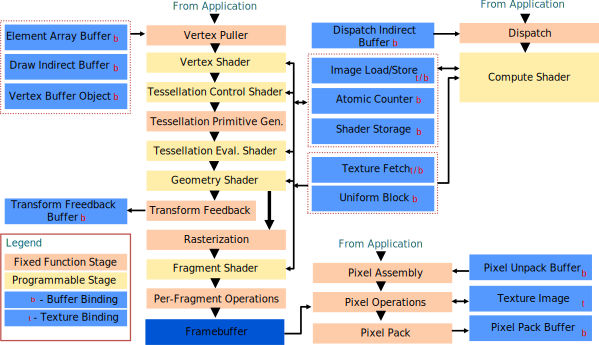
\includegraphics[width=11cm,keepaspectratio]{pics/opengl43.pdf}
	\end{figure}
\end{frame}

\begin{frame}[fragile]
\frametitle{Atomic counters/Shader Storage - example}
{\scriptsize
\begin{minted}[bgcolor=bg]{packages/graphics.py:GLShaderLexer -x}
#version 430

in vec4 vPos;

layout(binding=1,offset=0)uniform atomic_uint counter;
layout(std430,binding=0)buffer Output{vec4 data[];};

layout(location=0)vec4 fColor;
//...
void main(){
  int W=atomicCounterIncrement(counter);//increment counter
  data[w*2+0]=ComputeColor(...);//compute color
  data[w*2+1]=vPos;//write position
  //...
}
\end{minted}
}
\end{frame}

\begin{frame}[fragile]
\frametitle{Atomic counters/Shader Storage - example}
{\scriptsize
\begin{minted}[bgcolor=bg]{packages/c_cpp.py:CppLexer -x}
unsigned data[4]={0,0,0,0};
GLuint ACB;//identifier of a. counter
glCreateBuffers(1,&ACB);//create a. counter buffer
glNamedBufferData(ACB,sizeof(uint32_t)*4,data,GL_DYNAMIC_DRAW);
glBindBufferBase(GL_ATOMIC_COUNTER_BUFFER,1,ACB);//binding point 1

GLuint SSBO;//identifier of shader storage buffer
glCreateBuffers(1,&SSBO);//reserve identifier
glNamedBufferData(GL_SHADER_STORAGE_BUFFER,sizeof(float)*4*2*Max,
  NULL,GL_DYNAMIC_DRAW);
glClearNamedBufferData(SSBO,GL_R32F,GL_RED,GL_FLOAT,NULL);
glBindBufferRange(GL_SHADER_STORAGE_BUFFER,0,SSBO,0,
  sizeof(float)*4*2*Max);//binding point 0
\end{minted}
}
\end{frame}

